\documentclass{article}
\usepackage[utf8]{inputenc}
\usepackage{listings}
\usepackage{multimedia} % to embed movies in the PDF file
\usepackage{graphicx}
\usepackage{comment}
\usepackage[english]{babel}
\usepackage{amsmath}
\usepackage{amsfonts}
\usepackage{wrapfig}
\usepackage{multirow}
\usepackage{verbatim}
\usepackage{float}
\usepackage{cancel}
\usepackage{caption}
\usepackage{subcaption}
\usepackage{/home/cade/Homework/latex-defs}
\usepackage{/home/cade/Homework/jlcode}

\title{AMATH 586 Homework 1}
\author{Cade Ballew \#2120804}
\date{April 8, 2022}

\begin{document}
	
\maketitle
	
\section{Problem 1}
\subsection{Part a}
Using the Taylor series representation of the matrix exponential and assuming that we can differentiate termwise, %maybe add note about passing derivative
\begin{align*}
\frac{d}{dt}e^{tA}=\frac{d}{dt}\sum_{n=0}^\infty\frac{(tA)^n}{n!}=\sum_{n=0}^\infty A^n\frac{d}{dt}\frac{t^n}{n!}=\sum_{n=1}^{\infty}A^n\frac{t^{n-1}}{(n-1)!}
\end{align*}
because the derivative of the $n=0$ term is zero. Now, we reindex $n\to n-1$ to get 
\begin{align*}
\frac{d}{dt}e^{tA}=\sum_{n=0}^{\infty}A^{n+1}\frac{t^{n}}{n!}=A\sum_{n=0}^\infty\frac{(tA)^n}{n!}=Ae^{tA}.
\end{align*}
Additionally,
\begin{align*}
\frac{d}{dt}e^{tA}=\sum_{n=0}^{\infty}A^{n+1}\frac{t^{n}}{n!}=\left(\sum_{n=0}^\infty\frac{(tA)^n}{n!}\right)A=e^{tA}A.
\end{align*}

\subsection{Part b}
Now, consider $u(t) = e^{t A} \eta$ where $\eta$ is constant with respect to $t$. By part a,
\[
u'(t)=Ae^{t A} \eta=Au(t).
\]
Additionally, we have from the lecture notes that $e^{0A}=I$, so
\[
u(0)=e^{0A}\eta=I\eta=\eta.
\]
Thus, $u(t)$ satisfies the IVP
  \begin{align*}
	\begin{cases}
		u'(t) = A u(t),\\
		u(0) = \eta.
	\end{cases}
\end{align*}

\section{Problem 2}
Consider the system 
\begin{align*}
	\begin{cases}
		u_1'(t) = u_1(t),\\
		u_2'(t) = u_2(t). 
	\end{cases}
\end{align*}
Namely, we take $f(u(t))=Iu(t)=u(t)$. Now, consider 
\[
u_0=\begin{pmatrix}
	0\\1
\end{pmatrix},
\]
\[
v_0=\begin{pmatrix}
	1\\0
\end{pmatrix},
\]
and solve the systems 
  \begin{align*}
	\begin{cases}
		u'(t) = f(u(t)),\\
		u(0) = u_0,
	\end{cases}
	\begin{cases}
		v'(t) = f(v(t)),\\
		v(0) = v_0.
	\end{cases}
\end{align*}
Then, because the identity matrix is diagonal, we can use (D.30) to compute 
\begin{align*}
e^{tI}=\begin{pmatrix}
	e^{t} &0\\
	0 &e^t
\end{pmatrix},
\end{align*}
so problem 1 gives that 
\begin{align*}
	u(t)=e^{tI}u_0=\begin{pmatrix}
		e^{t} &0\\
		0 &e^t
	\end{pmatrix}\begin{pmatrix}
	0\\1
\end{pmatrix}=\begin{pmatrix}
0\\e^t
\end{pmatrix},
\end{align*}
and 
\begin{align*}
	v(t)=e^{tI}v_0=\begin{pmatrix}
	e^{t} &0\\
	0 &e^t
\end{pmatrix}\begin{pmatrix}
	1\\0
\end{pmatrix}=\begin{pmatrix}
	e^t\\0
\end{pmatrix}. 
\end{align*}
Then, using the homogeneity of norms and the positivity of $e^t$,
\begin{align*}
\|u(t) - v(t)\|_2 =\left\|\begin{pmatrix}
	0\\e^t
\end{pmatrix}-\begin{pmatrix}
e^t\\0
\end{pmatrix}\right\|_2=\left\|\begin{pmatrix}
-e^t\\e^t
\end{pmatrix}\right\|_2=e^t\left\|\begin{pmatrix}
-1\\1
\end{pmatrix}\right\|_2=e^t\left\|u_0-v_0\right\|_2,
\end{align*}
so we simply take $L=1$ and 
\begin{align*}
	\|u(t) - v(t)\|_2 = \|u(0) - v(0)\|_2 e^{L t}
\end{align*}
holds. Note that $L=1$ is a Lipschitz constant for $f$ as 
\[
\|f(u)-f(v)\|=\|u-v\|=L\|u-v\|
\]
for $L=1$. However, if we instead consider 
\begin{align*}
	\begin{cases}
	u'(t) = -f(u(t)),\\
	u(0) = u_0,
\end{cases}
\begin{cases}
	v'(t) = -f(v(t)),\\
	v(0) = v_0.
\end{cases}
\end{align*}
we now have 
\begin{align*}
	u(t)=e^{t(-I)}u_0=\begin{pmatrix}
		e^{-t} &0\\
		0 &e^{-t}
	\end{pmatrix}\begin{pmatrix}
		0\\1
	\end{pmatrix}=\begin{pmatrix}
		0\\e^{-t}
	\end{pmatrix},
\end{align*}
and 
\begin{align*}
	v(t)=e^{t(-I)}v_0=\begin{pmatrix}
		e^{-t} &0\\
		0 &e^{-t}
	\end{pmatrix}\begin{pmatrix}
		1\\0
	\end{pmatrix}=\begin{pmatrix}
		e^{-t}\\0
	\end{pmatrix},
\end{align*}
Then, 
we find that
\begin{align*}
	\|u(t) - v(t)\|_2 =\left\|\begin{pmatrix}
		-e^{-t}\\e^{-t}
	\end{pmatrix}\right\|_2=e^{-t}\left\|\begin{pmatrix}
		-1\\1
	\end{pmatrix}\right\|_2=e^{-t}\left\|u(0)-v(0)\right\|_2,
\end{align*}
Thus, in order for 
\begin{align*}
	e^{-t}\left\|u(0)-v(0)\right\|_2=\|u(t) - v(t)\|_2 = \|u(0) - v(0)\|_2 e^{L t}
\end{align*}
to hold, we need that $e^{(L+1)t}=1$. However, in order for this to be true for $t\neq0$, we need that $L=-1$ which implies that it is not a Lipschitz constant as a Lipschitz constant must be positive by definition. This means that this relation cannot hold no matter what the Lipschitz constant of $-f$ is.

\section{Problem 3}
Consider the IVP
\begin{align*}
	\begin{cases}
		u_1'(t) = 2u_1(t),\\
		u_2'(t) = 3u_1(t) - u_2(t),
	\end{cases}
\end{align*}
with initial conditions specified at time $t=0$. Denote these by $\eta_1$ and $\eta_2$, respectively.  
\subsection{Part a}
We first find that
\[
\frac{u'_1(t)}{u_1(t)}=2,
\]
so a general solution is given by $u_1(x)=ce^{2t}$ which becomes 
\[
u_1(t)=\eta_1e^{2t}
\]
when we implement our boundary condition. Inserting this into our other equation,
\[
u_2'(t) = 3\eta_1e^{2t} - u_2(t).
\]
Using (5.8), 
\begin{align*}
u_2(t)=e^{-t}\eta_2+\int_0^te^{\tau-t}3\eta_1e^{2\tau}d\tau=e^{-t}\eta_2+\eta_1\left[e^{3\tau-t}\right]_0^t=\eta_1(e^{2t}-e^{-t})+\eta_2e^{-t}.
\end{align*}

\subsection{Part b}
Now, consider 
\[
u(t)=\begin{pmatrix}
	u_1(t)\\u_2(t)
\end{pmatrix},
\]

\[
A=\begin{pmatrix}
	2 &0\\
	3 &-1
\end{pmatrix},
\]
and 
\[
\eta=\begin{pmatrix}
	\eta_1\\ \eta_2
\end{pmatrix}.
\]
Then, our IVP can be rewritten as
  \begin{align*}
	\begin{cases}
		u'(t) = A u(t),\\
		u(0) = \eta,
	\end{cases}
\end{align*}
so we can apply problem 1. To compute the matrix exponential using (D.30), note that\footnote{Obtained with the help of Mathematica}
\[
A=\begin{pmatrix}
	2 &0\\
	3 &-1
\end{pmatrix}=\begin{pmatrix}
1 &0\\
1 &1
\end{pmatrix}\begin{pmatrix}
2 &0\\
0 &-1
\end{pmatrix}\begin{pmatrix}
1 &0\\
-1 &1
\end{pmatrix}
\]
and that 
\[
\begin{pmatrix}
	1 &0\\
	1 &1
\end{pmatrix}\begin{pmatrix}
	1 &0\\
	-1 &1
\end{pmatrix}=\begin{pmatrix}
1 &0\\
0 &1
\end{pmatrix}.
\]
Then,
\begin{align*}
e^{tA}=\begin{pmatrix}
	1 &0\\
	1 &1
\end{pmatrix}\begin{pmatrix}
	e^{2t} &0\\
	0 &e^{-t}
\end{pmatrix}\begin{pmatrix}
	1 &0\\
	-1 &1
\end{pmatrix}=\begin{pmatrix}
e^{2t} &0\\
e^{2t}-e^{-t} &e^{-t}
\end{pmatrix}.
\end{align*}
Then, problem 1 gives that 
\begin{align*}
u(t)=e^{tA}\eta=\begin{pmatrix}
	e^{2t} &0\\
	e^{2t}-e^{-t} &e^{-t}
\end{pmatrix}\begin{pmatrix}
\eta_1\\ \eta_2
\end{pmatrix}=\begin{pmatrix}
\eta_1e^{2t}\\\eta_1(e^{2t}-e^{-t})+\eta_2e^{-t}
\end{pmatrix},
\end{align*}
so as in part a, 
\[
u_1(t)=\eta_1e^{2t},
\]
and
\begin{align*}
	u_2(t)=\eta_1(e^{2t}-e^{-t})+\eta_2e^{-t}.
\end{align*}

\section{Problem 4}
Now, consider the IVP
\begin{equation*}
	\begin{cases}
		u_1'(t) = 2u_1(t),\\
		u_2'(t) = 3u_1 + 2u_2(t)
	\end{cases}
\end{equation*}
with initial conditions specified at time $t=0$. We solve this using the method of problem 3 part a by again denoting these by $u_1(0)=\eta_1$ and $u_2(0)=\eta_2$ and noting that we have the same conditions on $u_1$ as before, so
\[
u_1(t)=\eta_1e^{2t}.
\]
Using (5.8),
\begin{align*}
	u_2(t)=e^{2t}\eta_2+\int_0^te^{2(t-\tau)}3\eta_1e^{2\tau}d\tau=e^{2t}\eta_2+3\eta_1e^{2t}\left[\tau\right]_0^t=3\eta_1te^{2t}+\eta_2e^{2t}.
\end{align*}

\section{Problem 5}
Consider the Lotka--Volterra system
\begin{align*}
	\begin{cases}
		u_1'(t) = \alpha u_1(t) - \beta u_1(t) u_2(t),\\
		u_2'(t) = \delta u_1(t) u_2(t) - \gamma u_2(t)
	\end{cases}
\end{align*}
for $\alpha = \delta = \gamma = \beta = 1$ and $u_1(0) = 5, u_2(0) = 0.8$. Using Julia, we approximate the solution with $k = 0.001$ for $t = 0,0.001,\ldots,50$ using both forward and backward Euler timesteps. We apply forward Euler by defining $$
f(u) = \begin{pmatrix} \alpha u_1(t) - \beta u_1(t) u_2(t) \\ \delta u_1(t) u_2(t) - \gamma u_2(t) \end{pmatrix}
$$ and taking the iteration 
\[
u^{n+1}=u^n+kf(u^n)
\]
at each timestep. This produces the following solution plots.\\
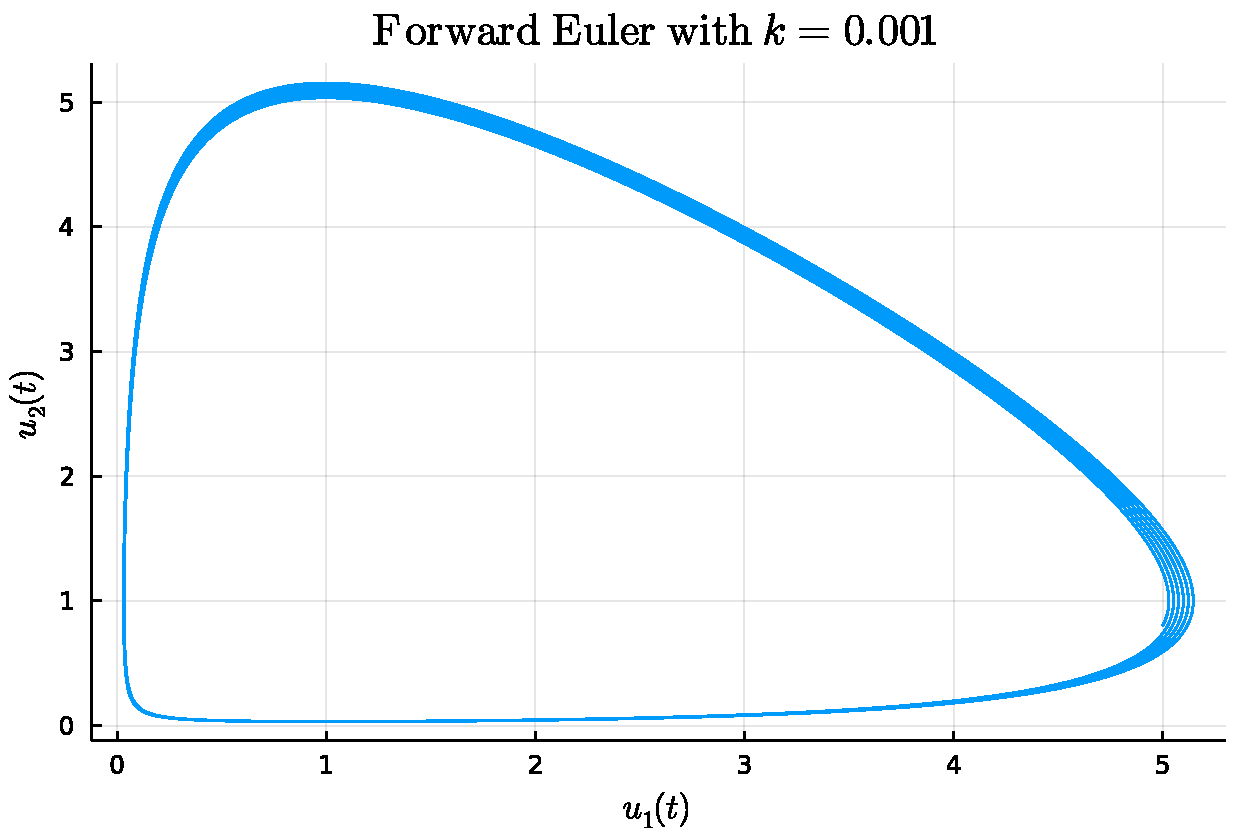
\includegraphics[scale=0.5]{fe1.pdf}\\
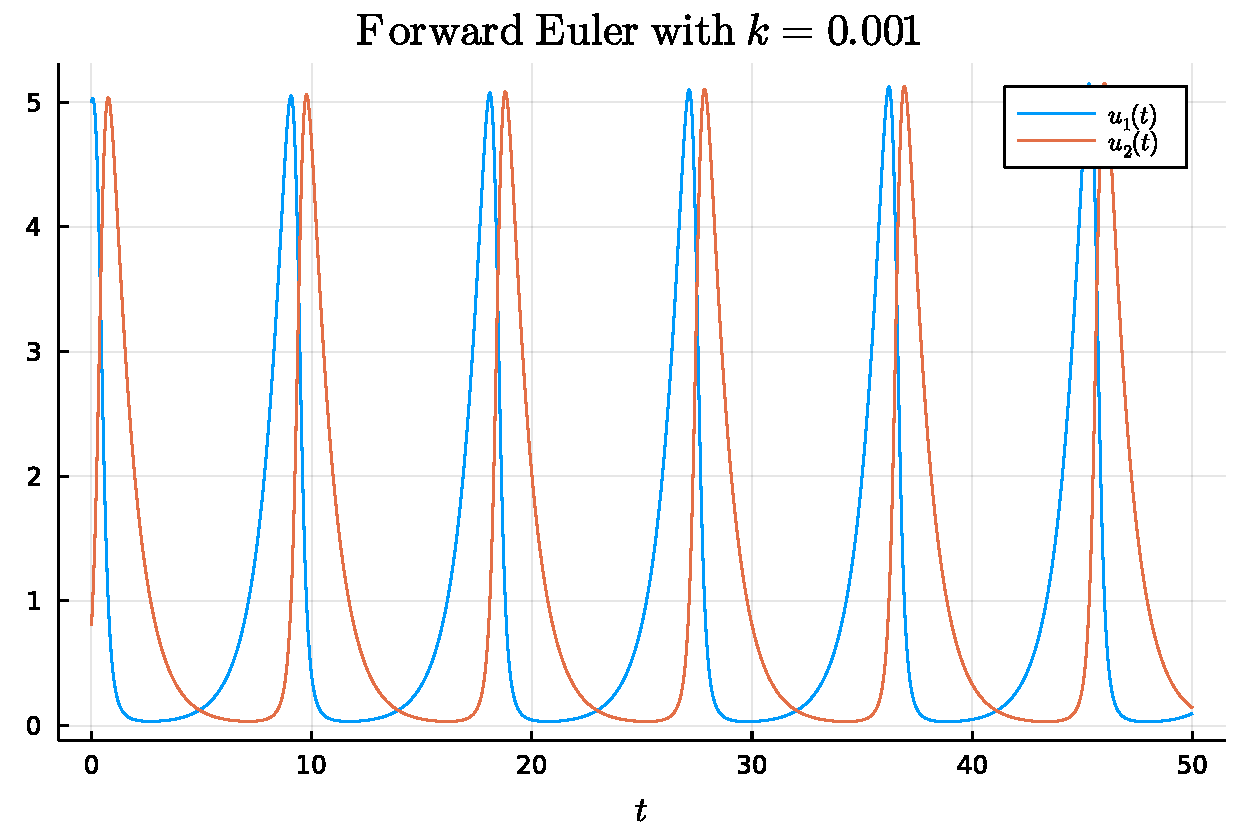
\includegraphics[scale=0.5]{fe2.pdf}\\
Applying backward Euler requires the iteration
\[
u^{n+1}=u^n+kf(u^{n+1})
\]
which requires us to define
\[
g(U) = u - u^n - kf(u)
\]
which has Jacobian
\[
D_u g(u) = \begin{pmatrix} 1+k(\alpha-\beta u_2(t)) & -k\beta u_1(t)\\ k\delta u_2(t) & 1+k(\delta u_1(t)-\gamma) \end{pmatrix}.
\]
This allows us to approximate the solution to $g(u)=0$ by taking Newton iterations
$$u^{n+1}_{0} = u^n$$
$$u^{n+1}_{k+1} = u^{n+1}_{k} - [D_u g(u^{n+1}_{k})]^{-1} g(u^{n+1}_{k}), ~~~k = 0,1,2,\ldots.$$
Doing this yields the following solution plots.\\
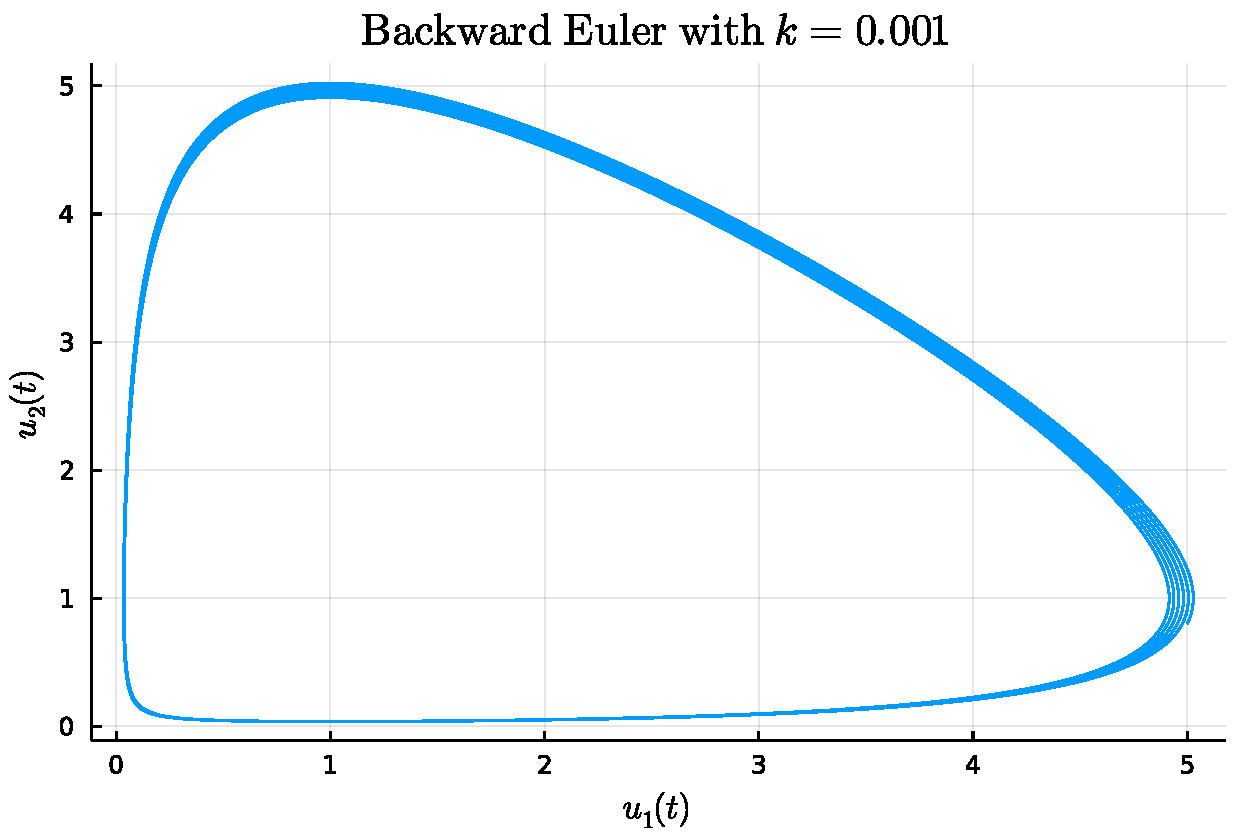
\includegraphics[scale=0.5]{be1.pdf}\\
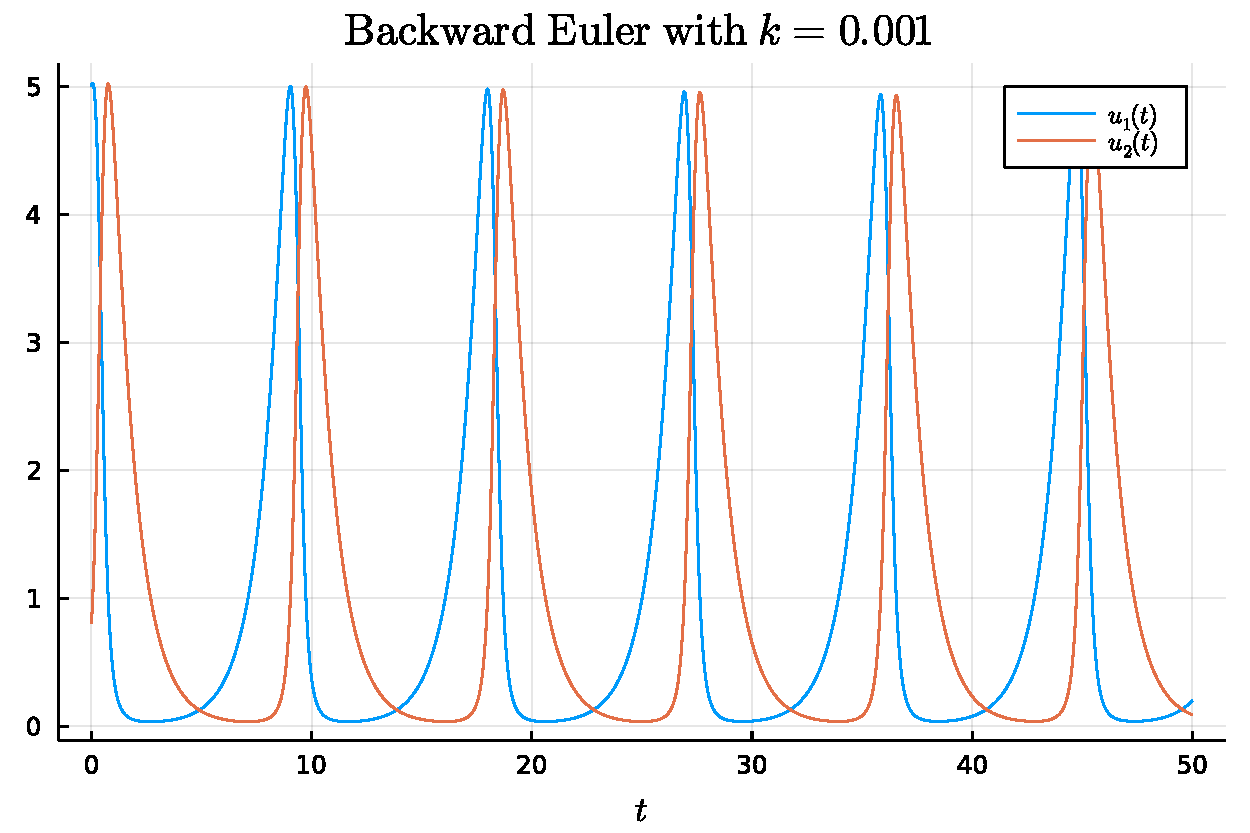
\includegraphics[scale=0.5]{be2.pdf}\\
The forward and backward plots look quite similar, but there is a subtle difference that one can observe in the $(u_1,u_2)$-plane; as time increases, the forward Euler solution appears to be spiraling outward while the backward Euler solution appears to be spiraling inward. What this suggests is that forward Euler is amplifying our solution while backward Euler is dampening it. This is consistent with the behavior we observed in class and suggests that neither method will be accurate in long time intervals. \\See Appendix A for the Julia code that produces these plots.

\section{Problem 6}
\subsection{Part a}
From (5.44), a 2-step LMM has form
\[
\alpha_0u^n+\alpha_1u^{n+1}+\alpha_2u^{n+2}=k\left(\beta_0f(u^n)+\beta_1f(u^{n+1})+\beta_2f(u^{n+2})\right).
\]
From (5.45), we know that the 2-step Adams-Moulton method takes $\alpha_0=0$, $\alpha_1=-1$, $\alpha_2=1$. Noting that these sum to zero, we can then compute the LTE using the formula on page 133 of the text. 
\begin{align*}
\tau_{n+2}&=\left(\sum_{j=0}^2(j\alpha_j-\beta_j)\right)u'(t_n)+k\left(\sum_{j=0}^2\left(\frac{1}{2}j^2\alpha_j-j\beta_j\right)\right)u''(t_n)\\&+k^2\left(\sum_{j=0}^2\left(\frac{1}{6}j^3\alpha_j-\frac{1}{2}j^2\beta_j\right)\right)u'''(t_n)+k^3\left(\sum_{j=0}^2\left(\frac{1}{24}j^4\alpha_j-\frac{1}{6}j^3\right)\right)u^{(4)}(t_n)+\OO(k^4)\\&=
(-1+2-\beta_0-\beta_1-\beta_2)u'(t_n)+k\left(\frac{-1}{2}+2-\beta_1-2\beta_2\right)u''(t_n)\\&+k^2\left(\frac{-1}{6}+\frac{4}{3}-\frac{1}{2}\beta_1-2\beta_2\right)u'''(t_n)+k^3\left(\frac{-1}{24}+\frac{2}{3}-\frac{1}{6}\beta_1-\frac{4}{3}\beta_2\right)u^{(4)}(t_n)+\OO(k^4).
\end{align*}
In order to achieve third order accuracy, we need the first three terms to each be zero. We can impose this condition as the following linear system. 
\[
\begin{pmatrix}
	1&1&1\\
	0&1&2\\
	0&\frac{1}{2}&2
\end{pmatrix}\begin{pmatrix}
\beta_0\\\beta_1\\\beta_2
\end{pmatrix}=\begin{pmatrix}
1\\3/2\\7/6
\end{pmatrix}.
\]
Solving this\footnote{Again with the help of Mathematica} yields solution
\[
\begin{pmatrix}
	\beta_0\\\beta_1\\\beta_2
\end{pmatrix}=\begin{pmatrix}
	-1/12\\
	2/3\\
5/12
\end{pmatrix}.
\]
One can verify that this is not higher order by noticing that the $k^3$ term in the above LTE does not vanish in general for these values of $\beta_j$. These values of $\alpha_j$ and $\beta_j$ yield the scheme 
\[
u^{n+2}=u^{n+1}+k\left(-\frac{1}{12}f(u^n)+\frac{2}{3}f(u^{n+1})+\frac{5}{12}f(u^{n+2})\right)
\]
which matches the two-step implicit Adams-Moulton method found on page 132 of the text.

\subsection{Part b}
Now, consider the three
times $t_n=-k$, $t_{n+1}=0$, and $t_{n+2}=k$ and polynomial
\[
p(t) = A + B(t+k) + C(t+k)t
\]
that we wish to interpolate through the three values
$f(U^n),~f(U^{n+1})$ and $f(U^{n+2})$ at these points. Then, the relation
\[
u(t_{n+2}) = u(t_{n+1}) + \int_{t_{n+1}}^{t_{n+2}}\,f(u(s))\,ds.
\]
can be applied to derive the approximation
\[
u^{n+2}=u^{n+1}+\int_{0}^{k}p(t)dt.
\]
We first determine the coefficients of $p(t)$ by setting
\[
f(u^n)=p(-k)=A,
\]
\[
f(u^{n+1})=p(0)=A+kB,
\]
and
\[
f(u^{n+2})=p(k)=A+kB+2k^2C.
\]
Solving these sequentially yields
\begin{align*}
&A = f(u^n),\\
&B=\frac{f(u^{n+1})-f(u^n)}{k},\\
&C=\frac{f(u^{n+2})-2f(u^{n+1})+f(u^n)}{2k^2}.
\end{align*}
Then,
\begin{align*}
\int_{0}^{k}p(t)dt&=\left[At+\frac{Bt^2}{2}+Btk+\frac{Ct^3}{3}+\frac{Ct^2k}{2}\right]_0^k=Ak+\frac{3B}{2}k^2+\frac{5C}{6}k^3\\&=
kf(u^n)+\frac{3k}{2}(f(u^{n+1})-f(u^n))+\frac{5k}{12}(f(u^{n+2})-2f(u^{n+1})+f(u^n))\\&=
k\left(\left(1-\frac{3}{2}+\frac{5}{12}\right)f(u^n)+\left(\frac{3}{2}-\frac{5}{6}\right)f(u^{n+1})+\frac{5}{12}f(u^{n+2})\right)\\&=
k\left(-\frac{1}{12}f(u^n)+\frac{2}{3}f(u^{n+1})+\frac{5}{12}f(u^{n+2})\right).
\end{align*}
Thus, our approximation is given by
\[
u^{n+2}=u^{n+1}+k\left(-\frac{1}{12}f(u^n)+\frac{2}{3}f(u^{n+1})+\frac{5}{12}f(u^{n+2})\right)
\]
which is the same as what we derived before. 

\section{Appendix A}
The following is displayed from Problem5.jl which is also in the Github repository. 
\jlinputlisting{Problem5.jl}

\end{document}
